\chapter{序論}
\thispagestyle{fancy}
\nobreak
\section{研究背景と目的}
本研究は「オーディトリウムの“底”で演奏を聴く」という旧態依然とした鑑賞形態並びにそれに基づく決定論的設計法に対し、建築音響学の観点から新たな息吹を吹き込むことで、次世代の建築を設計するための礎を築こうとするものである。

\subsection{2階バルコニー最前列席の音響的評価}
この世に存在する全てのオーディトリウムはいずれも室固有の響きを持っており、それは室を構成する形と内装条件によって決定づけられる。一般的な音響設計では、どの客席においても一様な反射音が到達するよう計画される。
ここで、収容人数や舞台へ向けての視野を確保する観点から、オーディトリウムにバルコニー席を設けることが多々ある。このとき、バルコニー先端部は前方に客席がなく、ホール空間へ張り出した特異な場となる。
\\ さて、2階バルコニー最前列の座席は、音響的に高い評価を得ることが多い$^{\text{\cite{01-1}}}$。これは、ホール空間が有する吸音力の大半(500Hzで7割程度)$^{\text{\cite{01-2}}}$を受け持っている1階客席床面(椅子+聴衆の吸音力)から相対的に離れた場所に位置するため、エネルギ減衰の少ない有効な直接音や反射音を得やすいことに起因すると定性的に推察されている(\textgt{図}\ref{fig:2階バルコニー最前列席の音場})。
\\
\\
\begin{figure}[h]
    \centering
    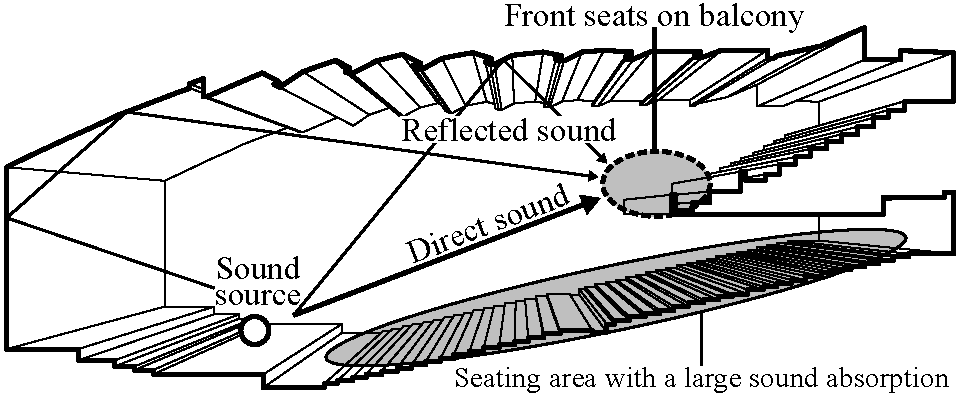
\includegraphics[keepaspectratio,scale=0.8]{01_att/second_balcony.pdf}
    \caption{\hspace{1mm}2階バルコニー最前列席の音場}
    \label{fig:2階バルコニー最前列席の音場}
\end{figure}

%-------------------------------------------------------------
\newpage
\subsection{評価対象領域の拡張}
美しい響きを生み出すにあたり、室容積は人間を収容するには冗長な大きさを要する。規模により異なるものの、室容積から算出されるホールの天井高はおおよそ10$\sim$20mである。ホール空間は人が鑑賞可能なエリアを断面方向含め無数に拡張できるというポテンシャルを秘めているにも関わらず、オーディトリウムの底で鑑賞をするという様式は依然として変わっていない。
\\ 建築音響学が体系化した1900年以後$^{\text{\cite{01-3}}}$、ホールの音響性能について種々研究が行われているものの、音場測定や解析シミュレーションによる音場の評価は、当然のことながら、建築的に確定された客席床面(床面上高さ1$\sim$2m)における面的評価に留まっており、ホール空間全体を評価対象とした設計研究は皆無である。本研究では、前節で述べた知見を踏まえ、評価対象領域を3次元的に拡張した評価を試みる(\textgt{図}\ref{fig:評価対象領域の拡張})。
\\
\begin{figure}[h]
    \centering
    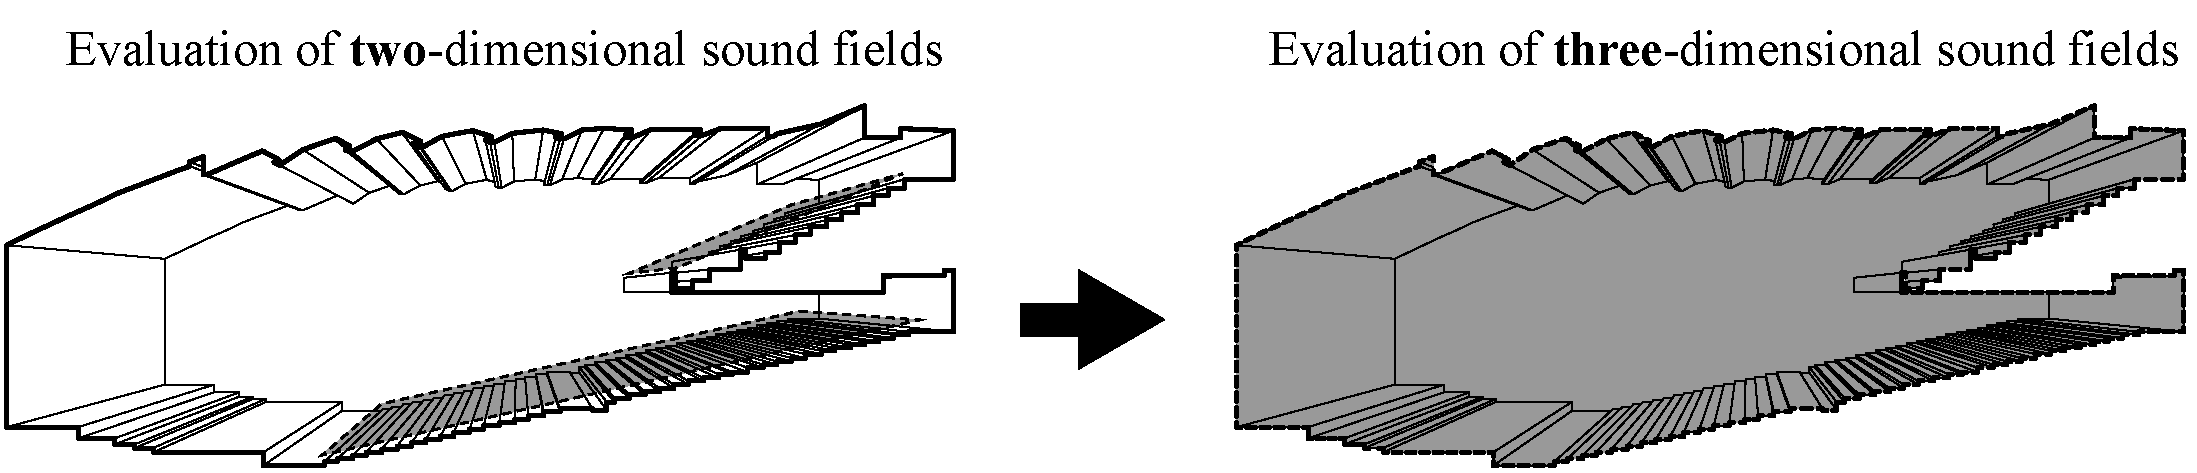
\includegraphics[keepaspectratio,scale=0.41]{01_att/evaluate_area.pdf}
    \caption{\hspace{1mm}評価対象領域の拡張}
    \label{fig:評価対象領域の拡張}
\end{figure}

\subsection{研究目的}
本研究は、コンサートホール音場の評価対象領域を、吸音力の大きな座席面近傍音場から3次元的に拡張し、座席面遠方音場(\textgt{図}\ref{fig:座席面遠方音場})の音響物理特性を明らかにすることにより、従来の面的評価並びにそれに基づく決定論的設計法に新たな可能性を見出すことを目的とするものである。
\\
\begin{figure}[h]
    \centering
    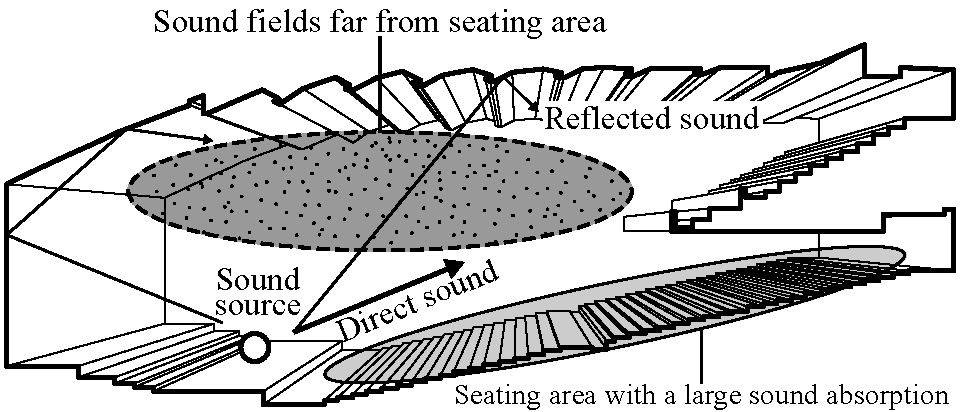
\includegraphics[keepaspectratio,scale=0.8]{01_att/zasekimen_enpo_English.pdf}
    \caption{\hspace{1mm}座席面遠方音場}
    \label{fig:座席面遠方音場}
\end{figure}

%-------------------------------------------------------------
\newpage
\section{既往の研究と本論の位置づけ}


\subsection{音環境の心理評価システム}
ある空間において音源から放射された音響信号を入力とし、その音響信号が作り出す音場に対する受聴者の主観評価を出力と捉えると、受聴者の心理評価システムは(\textgt{図}\ref{fig:室内音響心理評価システム})のように表すことができる$^{\text{\cite{森本政之1997室内音響心理評価のための物理指標}}}$。
音源から放射された信号$S(\omega)$は、室の壁や天井などによる反射、回折などの空間伝達関数$R(\omega)$の影響を受けて受聴者へ到達する。
さらに、この信号は頭部の影響を表す頭部伝達関数$HRTF_{l,r(\omega)}$の影響を受けて受聴者の左右の外耳道入口に到達し、心理空間への入力である音刺激となる。
心理空間において、受聴者は次に示す3つの性質に大別できる要素感覚(音を聴いた際に感じる基本的な感覚)をもった音像を知覚する。
\\(i)残響感などの時間的性質を有するもの。
\\(i\hspace{-.05em}i)方向感や広がり感などの空間的性質を有するもの。
\\(i\hspace{-.05em}i\hspace{-.05em}i)音量感や明瞭性、音色などの質的性質を有するもの。
\\ 受聴者はそれぞれの要素感覚に対して個人の嗜好に基づいた重みづけを行い、それらを総合し、総合主観評価を下す。
\\ 室内音響設計をするにあたり、「甘さ」を「砂糖(ショ糖)」の量で制御するように、要素感覚(心理量)を調整できる物理量並びに両者の関係を知ることが必要となる。コンサートホール等の音場の聴感印象に対応するとして定義された物理量を室内音響物理指標と呼び、目標とする音場はこの物理指標を用いることで客観的な設計が可能となる。\\

\begin{figure}[htbp]
    \centering
    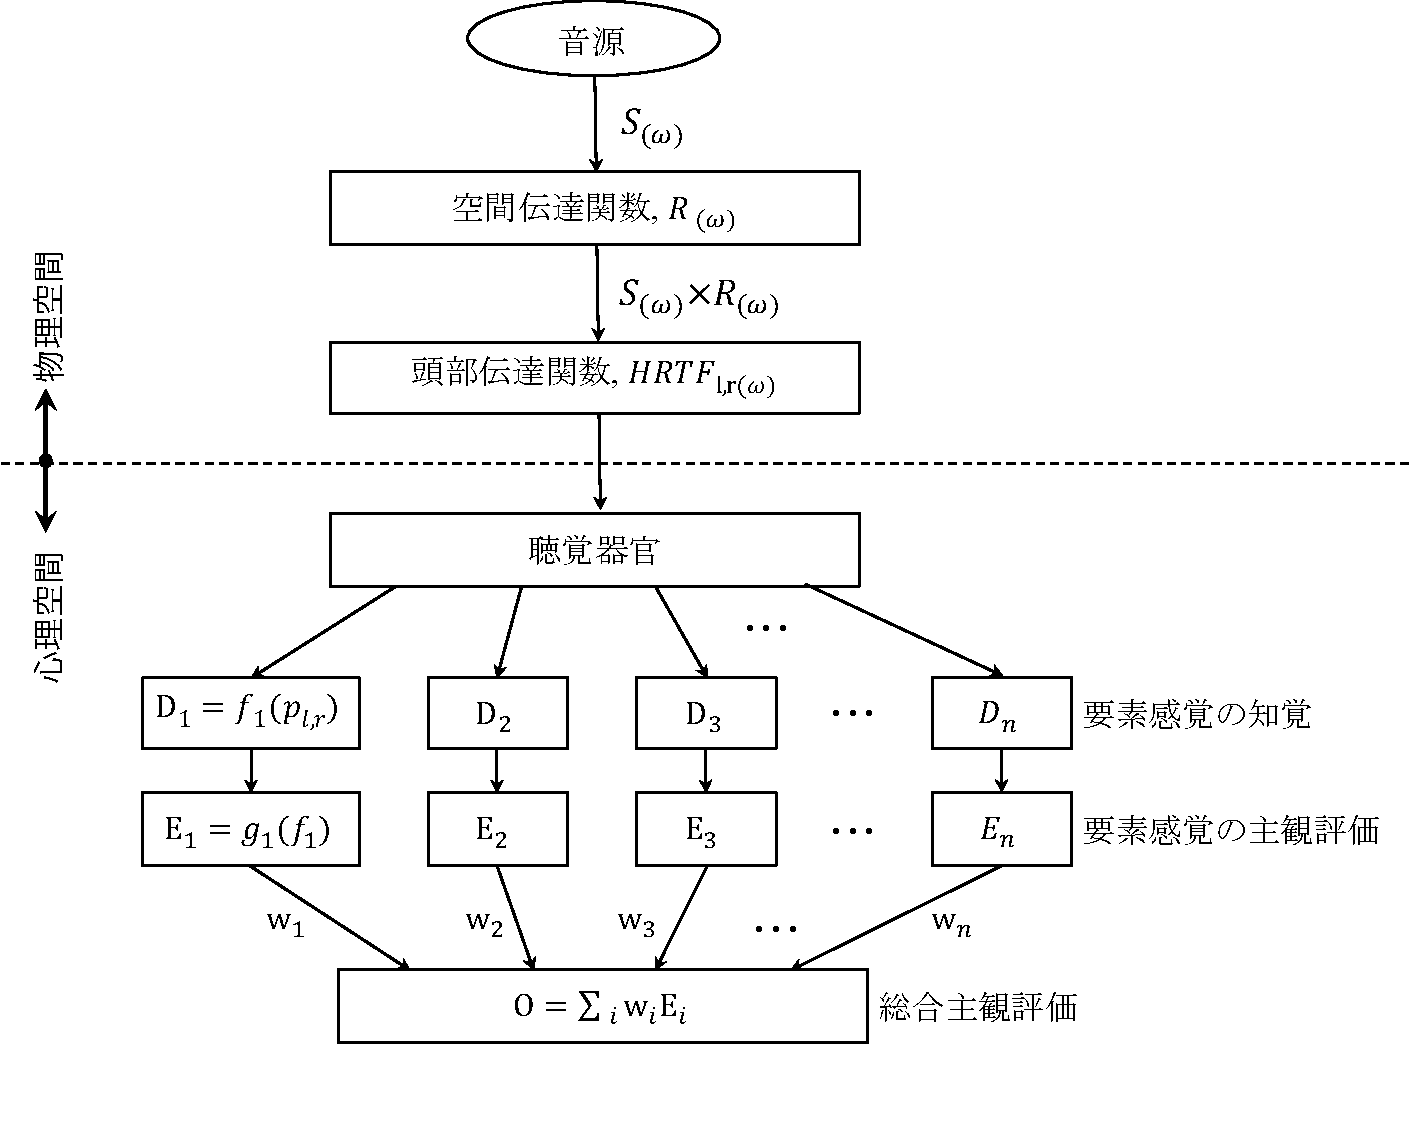
\includegraphics[keepaspectratio,scale=0.5]{01_att/phyco.pdf}
    \caption{\hspace{1mm}室内音響心理評価システム}
    \label{fig:室内音響心理評価システム}
\end{figure}

%-------------------------------------------------------------
\subsection{室内音響物理指標について}
ホール空間などにおいて特に重要な4つの要素感覚(音量感、残響感、明瞭性、広がり感)に対応するとして定義された、代表的な室内音響物理指標を以下に述べる$^{\text{\cite{01-3}}}$。

\subsubsection{音量感(Loudness)に対応する物理指標}
音の大きさは、到来する音の全エネルギー量に対応するとして、\STG が \textgt{式}\ref{eq:STG}より定義されている。これは、直接音を含む全ての反射音エネルギーを、音源のパワーに準ずるエネルギーによって基準化した量である。ここで、$p(t)$は観測点における音圧、$p_{A10}(t)$は無響室内10m点における音圧である。受聴レベルは、音量感だけでなく広がり感や残響感の大小にも影響を与えることが知られており、室内音場の性質を表す基本的かつ重要な物理指標である。

\begin{equation}
  \label{eq:STG}
  G = 10\log_{10}{\frac{\displaystyle\int_0^{\infty}p^2(t)dt}{\displaystyle\int_0^{\infty}p_{A10}^2(t)dt}} \dB
\end{equation}

\subsubsection{残響感(Reverberance)に対応する物理指標}
聴感的な響きの長さは、残響過程の比較的初期の減衰の仕方に影響を受けることが明らかにされており、初期残響時間EDT[s]が残響感に対応する物理指標として提案されている。これは、残響時間が60dB減衰に要する時間であるのに対し、初期の10dB減衰の傾きから算出した残響時間であり、10dB減衰に要する時間を6倍にしたものとして算出される。

\subsubsection{明瞭性(Clarity)に対応する物理指標}
初期反射音は、直接音をエネルギー的に補強し聴感的な明瞭性を高める効果がある。そこで、この初期反射音のエネルギーに着目し、音楽の明瞭度に対応する物理指標として初期/ 後期エネルギー比 \Clarity(Clarity) が\textgt{式}\ref{eq:c80}により定義されている。これは、初期反射音以外のエネルギー(t=80ms$\sim\infty$、後期反射音)に対する初期反射音エネルギー(t=0$\sim$80ms:直接音を含む)の割合をデシベル表示したものである。初期反射音エネルギーが増加するほど値は大きくなり、聴感的な明瞭性が増すことを意味する。

\begin{equation}
    \label{eq:c80}
  C_{80} = 10\log_{10}{\frac{\displaystyle\int_0^{80}p^2(t)dt}{\displaystyle\int_0^{\infty}p^2(t)dt}} \dB
\end{equation}

\subsubsection{広がり感(Spatial impression)に対応する物理指標}
室内では、さまざまな方向から反射音が到来する。これらの反射音のうち、両耳の方向から到来する反射音(側方反射音 : lateral reflection)が広がり感の知覚に強く関係している。
この側方エネルギー成分に着目し、みかけの音源の幅(ASW)に対応する物理指標として初期側方反射エネルギー率LF(Lateral energy fraction)が\textgt{式}\ref{eq:lf}により提案されている。ここで、$p(t)$は観測点における音圧、$\theta$は反射波の入射方向と受聴者の両耳軸のなす角度(真横 : $\theta = 0^\circ$、正面 : $\theta = 90^\circ$)である。

\begin{equation}
    \label{eq:lf}
  LF = \frac{\displaystyle\int_5^{80}p^2(t)cos{\theta}dt}{\displaystyle\int_0^{80}p^2(t)dt} \dB
\end{equation}


%-------------------------------------------------------------
\pagebreak
\subsection{フライングバルコニーを有するホールの事例}
Philharmonie de Parisを例にフライングバルコニーの紹介、本研究のテーマに近いホールがあることを示し、本テーマは突拍子もないことではないことを示す。
%-------------------------------------------------------------
\pagebreak
\subsection{本論の位置づけ}
前節でも述べた通り、ホール空間は吸音面が1階客席面に偏在する非完全拡散音場である。
ここで、座席面遠方音場は大きな吸音力を持つ座席面から離れることにより、反射音到来方向の偏りが是正されるという推測のもと、拡散性の観点から評価を行う。
室内音響学としての「拡散」に対応した心理的評価に関しては未だ研究の途上にあり、聴感印象に対応した指標は確立していない。
\\ さて、関連した用語として従来より残響理論の仮定として用いられる「完全拡散音場」がある。これは、次の2条件を満たす音場のことである。
\\(i)音響エネルギが室内全体に 均一に分布していること。
\\(i\hspace{-.05em}i)どの点においても音の進行方向があらゆる方向に一様であること。
\\ 完全拡散音場は音像が定位せず、聴感的に好ましくないとされる音場ではあるが、物理的な拡散性を言及するにあたり上記2条件を拡散性評価の参考とする。
\\ 以上を踏まえ、本研究では室内音響物理指標のみならず、音場の物理的評価に立脚した拡散性の観点からの評価も行う。
%-------------------------------------------------------------
%-------------------------------------------------------------
\section{論文構成}
本論文は、以下に示す全7章で構成される。
\\ 第1章では前節までに本研究の背景と目的、関連する既往研究の概要、本論の位置づけについて述べた。本節では、論文の構成について述べている。
\\ 第2章では、研究手法である幾何音響解析の概要、解析条件並びに解析モデルについて述べる。
\\ 第3章では、解析で得られたデータから残響特性の観点から音場評価を行う。
\\ 第4章では、時間エネルギ特性の観点から音場評価を行う。
\\ 第5章では、反射音方向分布特性の観点から距離減衰特性及び方向別エネルギ率の観点から音場評価を行う。
\\ 第6章では、これまでの研究結果を踏まえ、ホール形状の設計例を提示する。
\\ 最後の第7章では、本論文の結論を述べる。
